\section{Experiments}

\subsection{Introduction to the tools}
\subsubsection{Python (\texttt{regex})}
The \texttt{regex}\footnote{\url{https://pypi.python.org/pypi/regex}} Python
module is intended to replace the current \texttt{re} module at some point. It
is a fairly fully fledged regular expression module, that also supports
approximate matching. Because of this and the ease of creating the necessary
scripts we chose to include it in the benchmarks. Unfortunately, there is
little information, other that the source code, about the theoretical
background or the inner workings of this implementation.

\subsubsection{Approximate Kleenex}
Approximate matching was introduced to Kleenex by P. Troelsen in his master's
thesis~\cite{troelsen2016approximate}. As discussed previously, this is
accomplished by rewriting the core program terms to allow for a given number of
errors in the match, that is, to express the approximate matching as exact
matching.

\subsubsection{Scan For Matches}
Scan For Matches\footnote{\url{http://blog.theseed.org/servers/2010/07/scan-for-matches.html}}
(SFM)~\cite{dsouza1997searching} is an approximate pattern matching tool
specifically designed for matching biological sequences such as DNA, RNA, and
protein. It is written in C and has a bunch of nucleotide and protein specific
niceties that the other tools do not, such as using FASTA files directly, and
support for matching reverse complements (matching the DNA complement of a
previously occurred substring in reverse, e.g. corresponding to an RNA hairpin
loop).

\subsubsection{NR-grep}
NR-grep~\cite{navarro2001nr} is a fast pattern matching tool, similar to
\texttt{grep}, that is made to be efficient for complex pattern, and it also
supports approximate matching.


\subsection{Experiment setup and benchmark description}
The experiments where run on the \texttt{gpu02} machine.
\begin{description}
    \item[CPU] Intel Xeon E5-2650 v2 (2.60 GHz).
    \item[RAM] 128 GB.
    \item[Disk] KU network share.
\end{description}

The data set used for the benchmark is from
\url{ftp://ftp-trace.ncbi.nih.gov/1000genomes/ftp/technical/reference/human_g1k_v37.fasta.gz}
and is 2.9 GBs uncompressed, for most of the benchmarks we used a file where we
stripped the newlines, so they would not count as an error, except for the
NR-grep trails since it was not too happy about lines longer than $2^{16}$.

\subsubsection{Patterns used}
We have made a number of patterns to benchmark the different tools, they are
represented here in the Kleenex syntax, with $k$ being the allowed number of
substitutions going from 0 up to 5 (if possible). They are not all possible in
all of the tools, only Kleenex has support for all the patterns. Also we search
for the pattern, not just plain string matching, so in Kleenex we had to add an
alternation and a star, to discard any input that did not match the pattern.

\texttt{/TGCAAGCGTTAAT/<$k$>} - Short - A simple fairly short pattern with
nothing but a character string.

\texttt{/GCCCAGAGAACTTTCAGGATGACACCAGCAAGG/<$k$>} - Long - A longer simple
pattern it is only 33 characters long because it was the longest we could
compile a Kleenex program for with $k \leq 2$

\texttt{(/GCCCAGAGA/|/ACTTTCAGGA/)<$k$>} - Alternation - An alternation with a
simple fairly short pattern on each side of the alternation.

\texttt{(/[ACGT]/\{5,15\} /TGCAAGCGTTAAT/)<k>} - Ranges - A small pattern with
a ranges of repetitions, followed by another fairly short pattern.

\subsection{Results}
In Figure \ref{fig:short}, we have the runtimes for the \textit{Short} pattern
with the different tools. What we see is that \texttt{regex} seems to be quite
far outmatched by all the other tools, which seems to by a general thing, the
cause for being so far behind, can probably partly be blamed on the Python
scripts read the entire file in to memory before beginning to search for the
pattern. But overall \texttt{regex} does not seem to have too bad a complexity
with respect to $k$. For the rest of the tools they are fairly close in
performance with SFM being the worst in low $k$ but having a seemingly near
constant complexity with respect to $k$ and performing better for larger $k$.
NR-grep while having the advantage of not having a single line file, gives the
best results here for smaller $k$, but does have some wiered behaviour with it
being better for $k=5$ and for $k=4$. Finally Kleenex performes quite well
beating out SFM but not NR-grep, to begin with, but does really bad once we hit
$k=3$, the reason for this sudden performance hit is likely due to caching
issues, that are grounded in the executable size being 11MB.

Figures \ref{fig:long} and \ref{fig:alternation} show fairly similar results to
to that of Figure \ref{fig:short}, which suggest that none of the tools do
anything special that would change their relative performace.

Finally Figure \ref{fig:ranges} show Kleenex performing quite bad when having a
range to match, especially when the large executable size for $k=1$ kicks in.
Whereas \texttt{regex} has a similar performance to the other benchmarks.

\begin{figure}[!ht]
  \centering
  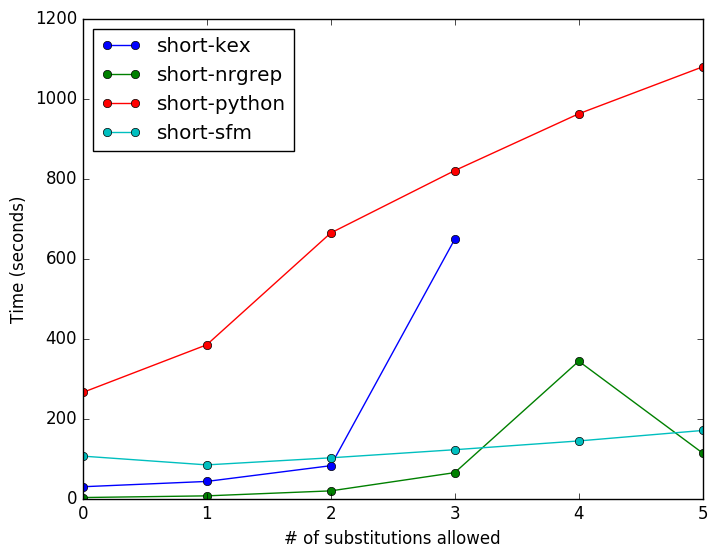
\includegraphics[width=0.9\textwidth]{images/short.png}
  \caption{Execution times for approximate Kleenex, NR-grep, Python's
    \texttt{regex} module, and \texttt{scan\_for\_matches}, when searching for
    the pattern \texttt{/TGCAAGCGTTAAT/<$k$>} for $k=0..5$.}
  \label{fig:short}
\end{figure}

\begin{figure}[!ht]
  \centering
  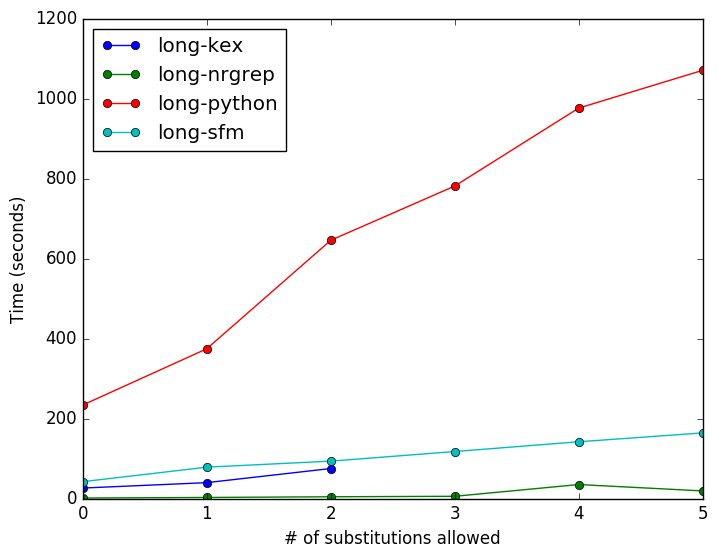
\includegraphics[width=0.9\textwidth]{images/long.png}
  \caption{Execution times for the evaluated tools when searching for the
    pattern \texttt{/GCCCAGAGAACTTTCAGGATGACACCAGCAAGG/<$k$>} for $k=0..5$.}
  \label{fig:long}
\end{figure}

\begin{figure}[!ht]
  \centering
  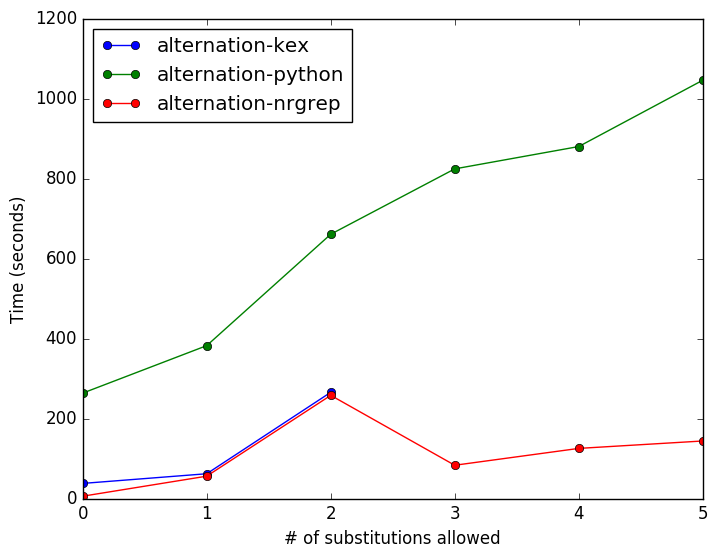
\includegraphics[width=0.9\textwidth]{images/alternation.png}
  \caption{Execution times for the evaluated tools when searching for the
    pattern \texttt{(/GCCCAGAGA/|/ACTTTCAGGA/)<$k$>} for $k=0..5$.}
  \label{fig:alternation}
\end{figure}

\begin{figure}[!ht]
  \centering
  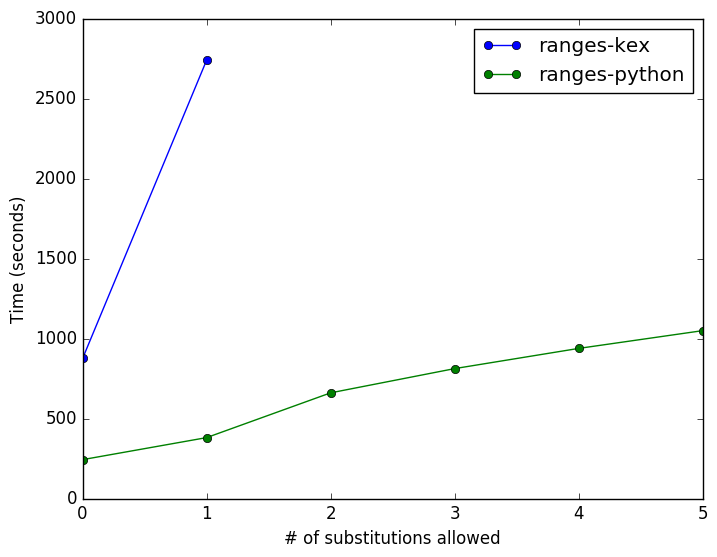
\includegraphics[width=0.9\textwidth]{images/ranges.png}
  \caption{Execution times for the evaluated tools when searching for the
    pattern \texttt{(/[ACGT]/\{5,15\} /TGCAAGCGTTAAT/)<$k$>} for $k=0..5$.}
  \label{fig:ranges}
\end{figure}

\begin{figure}[!ht]
    \centering
    \begin{tabular}{l|rrrrr}
                    & 0     & 1     & 2     & 3\\\hline
        Short       & 23    & 89    & 716   & 11,000\\
        Long        & 23    & 192   & 1,700 & N/A\\
        Alternation & 32    & 234   & 2,800 & N/A\\
        Ranges      & 92    & 21,000& N/A   & N/A\\
    \end{tabular}
    \caption{Size(KB) of the executables generated by Kleenex for the patterns
    and different $k$.}
    \label{fig:exec}
\end{figure}

\subsubsection{Remarks}
NR-grep is capable of searching in lines that are longer than $2^{16}$ but it
outputs a bunch of warnings cluttering output, and also has some wierd runtimes
as seen in Figure \ref{fig:nr-longline}, and this is without having checked if
it finds the correct number of matches.

Also SFM does not seem to support approximate matching for alternations, as we
could not get the pattern to compile with the error values added.

\begin{figure}[!ht]
    \centering
    \begin{tabular}{l|rrrrr}
        $k$ & Time (s)\\\hline
        0   & 4.59\\
        1   & 43.32\\
        2   & 1185.80\\
        3   & 1323.27\\
        4   & 906.27\\
        5   & 30.04\\
    \end{tabular}
    \caption{Run time for NR-grep with a single long line.}
    \label{fig:nr-longline}
\end{figure}


%%% Local Variables:
%%% mode: latex
%%% TeX-master: "main"
%%% End:
